\section{\algfullname}
\label{sec:zconv-intro}

\algfullname (\algname) is a novel convolution algorithm for CPUs designed around the key insight that all data copies required by traditional Im2col-based approaches can be eliminated.
This is achieved by decomposing the convolution into multiple GEMM calls and leveraging the GEMM API to operate on non-contiguous input matrices.
\algname's performance relies on heavily optimized GEMM kernels, making its algorithm simple and compatible with most architectures via open-source or vendor-specific BLAS libraries.
\algname supports all convolution parameters used in PyTorch's \emph{Conv2D} operator (listed in \rtab{conv-parameters}), except for the padding mode, which is fixed to zero-padding.
To provide this support, \algname includes two versions: a zero-copy implementation that covers most common configurations (\rsec{zconv-alg}), and an extended version that introduces a small copy step to support grouped and dilated convolutions (Appendix \ref{appendix:zconv-alg-ext}).
The start of \ralg{zconv} specifies the required tensor layouts for \algname, which are commonly found in frameworks such as PyTorch~\cite{pytorch2024} and TensorFlow~\cite{tensorflow}. 
To execute \algname in end-to-end models, its algorithm was integrated into PyTorch, as described in \rsec{pytorch-integration}.

\subsection{\algname Algorithm}
\label{sec:zconv-alg}

In \ralg{zconv}, \algname is described; its parameters are given in \rtab{conv-parameters}.
The two outermost loops iterate over the batch (\texttt{N}) and output width (\texttt{OW}), which correspond to the first and third dimensions of the output tensor.
Each iteration of these loops computes a distinct output tile of shape \texttt{[OH,1,OC]}, allowing them to be parallelized.
Lines~\ref{alg:zconv:initialize-start}-\ref{alg:zconv:initialize-end} initialize the output tile to the corresponding bias values (or to zero if there is no bias).
The only remaining loop, at Line~\ref{alg:zconv:fh}, iterates over the filter height (\texttt{FH}), setting the appropriate GEMM parameters and calling GEMM.
Each iteration over the filter height computes a partial result for the \texttt{[OH,1,OC]} output tile.
GEMM is called in row-major layout, with input matrices used as-is (\ie, no transposition), and with scalar multipliers \texttt{alpha} and \texttt{beta} both set to one.
Line~\ref{alg:zconv:dims} describes the GEMM dimensions \emph{m}, \emph{n}, and \emph{k} typically used in \algname.
An example of these matrix tiles within the convolution tensors is highlighted in \rfig{tensors}.
Overall, GEMM is invoked $\texttt{N}\times\texttt{OW}\times\texttt{FH}$ times.

Padding is omitted from \ralg{zconv} for readability.
Convolution with padding is handled in \algname by skipping accesses to padding elements, resulting in GEMM calls with smaller matrices at the image edges.
Padding elements can be skipped and never instantiated in temporary buffers because the padding mode is fixed to zero-padding in \algname.
This is the default mode in PyTorch.
A full implementation with padding handling will be provided in the artifact.

\begin{algorithm}[t]
\caption{\algname (padding omitted for brevity).}
\label{alg:zconv}
\small
\begin{algorithmic}[1]
\Require
\begin{tabular}[t]{@{}ll@{}}
  $image[\texttt{N},\texttt{IH},\texttt{IW},\texttt{IC}]$, & $filter[\texttt{FH},\texttt{FW},\texttt{IC},\texttt{OC}]$ \\
  $output[\texttt{N},\texttt{OH},\texttt{OW},\texttt{OC}]$, & $bias[\texttt{OC}]$
\end{tabular}

\For{$n \gets 0$ to $\texttt{N}-1$} \Comment{Parallel loop}
  \For{$ow \gets 0$ to $\texttt{OW}-1$} \Comment{Parallel loop} \label{alg:zconv:ow}
    \For{$oh \gets 0$ to $\texttt{OH}-1$}   \label{alg:zconv:initialize-start}
      \For{$oc \gets 0$ to $\texttt{OC}-1$}
        \State $output[n,oh,ow,oc] \gets bias[oc]$
      \EndFor
    \EndFor  \label{alg:zconv:initialize-end}

    \For{$fh \gets 0$ to $\texttt{FH}-1$}  \label{alg:zconv:fh}
      \State $A \gets \text{addr}(image[n, fh, ow \cdot \texttt{SW}, 0])$ \label{alg:zconv:params-start}
      \State $B \gets \text{addr}(filter[fh,0,0,0])$
      \State $C \gets \text{addr}(output[n,0,ow,0])$
      \State $layout \gets rowMajor$
      \State $transa \gets noTrans,\;\; transb \gets noTrans$
      \State $m \gets \texttt{OH},\;\; k \gets \texttt{FW} \cdot \texttt{IC},\;\; n \gets \texttt{OC}$ \label{alg:zconv:dims}
      \State $lda \gets \texttt{IW} \cdot \texttt{IC} \cdot \texttt{SH},\;\; ldb \gets n,\;\; ldc \gets \texttt{OW} \cdot \texttt{OC}$
      \State $\alpha \gets 1,\;\; \beta \gets 1$ \label{alg:zconv:params-end}
      \State $C \gets \alpha A B + \beta C$\Comment{GEMM call}
    \EndFor
  \EndFor
\EndFor
\end{algorithmic}
\end{algorithm}

\rfig{zconv-simple} illustrates the example of the \algname algorithm with the convolution parameters detailed in its caption.
The figure expands the iterations over output width and filter height, corresponding to Lines~\ref{alg:zconv:ow} and \ref{alg:zconv:fh} of \ralg{zconv}.
The highlighted tiles in the image and filter represent the elements accessed during each iteration, which serve as inputs to the GEMM operation shown on the right side of the figure.
This GEMM accumulates its result into the corresponding tile of the output.
No data copies are involved in selecting the GEMM input tiles \textemdash these tiles are determined using a combination of their base pointers, matrix dimensions, and leading dimensions.

Intuitively, each GEMM call in \algname is equivalent to sliding a single filter row vertically across the image.
In \rfig{zconv-simple}, the first filter row is never multiplied with the elements of the last image row, which is why the image tiles do not cover the full column height in this example.
Similarly, the second filter row is not multiplied with the elements of the first image row.
The horizontal iterations in the image follow the width stride.

\begin{figure}[t]
    \centering
    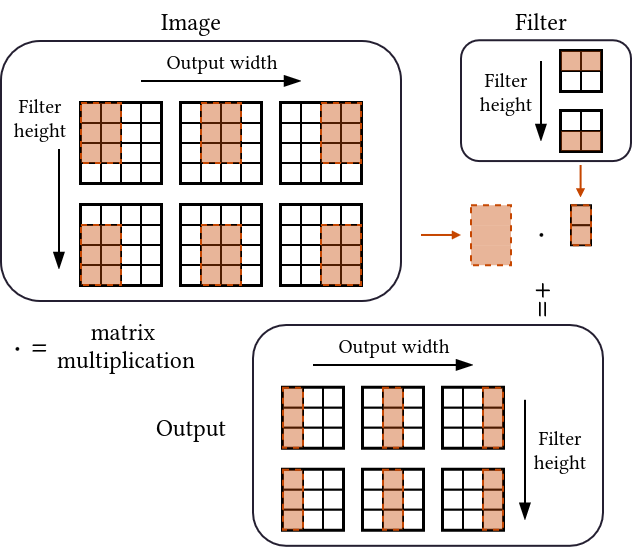
\includegraphics[width=0.9\columnwidth]{figures/zconv-column.png}
    % \Description{A four by four image matrix, two by two filter matrix, and a three by three output matrix. A tile of size OH by FW is highlighted over the image matrix, and it slides over the image height and width in increments of one. Vertically, these tiles represent iterations of the filter height loop. Horizontally, these tiles represent iterations in the output width loop. A tile of size 1 by FW slides over the filter matrix, representing the filter height loop iterations. The image and filter tiles are connected by a matrix multiplication operation. The output matrix has tiles of size OH by 1 highlighted, they move horizontally with the output width iterations, but do not change vertically with the filter height iterations.}
    \caption{View of \algname in a simplified convolution that uses unit stride, no padding, no dilation, and a $2\times2$ filter. 
    The tensors have only height and width dimensions, the image is $4\times4$, and the output is $3\times3$.
    Black arrows indicate loop iterations, and colors indicate the data flow.}
    \label{fig:zconv-simple}
\end{figure}

\ralg{zconv} sets the GEMM parameters in Lines~\ref{alg:zconv:params-start}-\ref{alg:zconv:params-end}.
Matrix $A$ points to the beginning of an \texttt{[OH,FW$\times$IC]} tile of the image tensor.
Matrix $A$ is a non-contiguous tile, where each row contains $\texttt{FW}\times\texttt{IC}$ contiguous elements, and the \texttt{lda} parameter specifies the stride between rows.
For example, in \rfig{zconv-simple}, the highlighted tiles from the image tensor are obtained with: $m\gets3$, $k\gets2$, and $lda\gets4$.
The value of $lda$ represents the stride in memory between the rows of the image tiles.
The algorithm naturally produces a matrix $C$ of shape \texttt{[OH,OC]}.
While this matrix could be stored as a contiguous tile in the output tensor, it would cause the output to have a transposed layout where the \texttt{OH} and \texttt{OW} dimensions are swapped.
Matrix $C$ is stored as a non-contiguous tile (using the $ldc$ parameter) to avoid this transposed layout.
In contrast, matrix $B$ is a contiguous tile from the filter tensor.
Although the filter tile in \rfig{zconv-simple} looks transposed, matrix $B$ does not require transposition because a single row and a single column both appear as contiguous arrays in memory.
This remains true for the algorithm when considering the additional filter dimensions.

\subsection{Integration of \algname with PyTorch}
\label{sec:pytorch-integration}

PyTorch~\cite{pytorch2024} supports multiple convolution backends and includes a selector that chooses between them, generally based on convolution parameters~\cite{adversarial-linear-algebra-backends2025}.
\algname was integrated as a new backend that is selected when the following conditions are met in end-to-end vision models:
\begin{enumerate*}[label=(\roman*)] 
    \item BLAS libraries are enabled (to provide a GEMM implementation).
    \item The input image uses the channel-last layout \texttt{[N,IH,IW,IC]}~\cite{pytorchChannelLast}, matching the layout expected by \algname.
    \item The convolution is not grouped ($\texttt{GR} = 1$), not pointwise ($\texttt{FH} \neq 1 \lor \texttt{FW} \neq 1$), and both output height and width dimensions are smaller than the number of input channels ($\texttt{OH} < \texttt{IC} \land \texttt{OW} < \texttt{IC}$).
\end{enumerate*}
The motivation for this heuristic is described in \rsec{libtorch}.
A search-based approach could further refine this heuristic, but it is out of the scope of this paper.

The filter tensor in the PyTorch channel-last layout \texttt{[OC,FH,FW,IC]} differs from the layout used by \algname, \texttt{[FH,FW,IC,OC]}.
To use the \algname backend, the filter tensor must be transformed.
This transformation can be performed either once ahead-of-time when converting the model to the channel-last format or before each invocation of a \algname convolution.
The end-to-end model evaluation performs the layout transformation ahead of time (\rsec{end-to-end}).